\documentclass[journal,onecolumn]{IEEEtran}
\usepackage{amsmath}
\usepackage[hidelinks]{hyperref}
\usepackage{graphicx}

% *** GRAPHICS RELATED PACKAGES ***
%
\ifCLASSINFOpdf
  % \usepackage[pdftex]{graphicx}
  % declare the path(s) where your graphic files are
  % \graphicspath{{../pdf/}{../jpeg/}}
  % and their extensions so you won't have to specify these with
  % every instance of \includegraphics
  % \DeclareGraphicsExtensions{.pdf,.jpeg,.png}
\else
  % or other class option (dvipsone, dvipdf, if not using dvips). graphicx
  % will default to the driver specified in the system graphics.cfg if no
  % driver is specified.
  % \usepackage[dvips]{graphicx}
  % declare the path(s) where your graphic files are
  % \graphicspath{{../eps/}}
  % and their extensions so you won't have to specify these with
  % every instance of \includegraphics
  % \DeclareGraphicsExtensions{.eps}
\fi

% correct bad hyphenation here
\hyphenation{op-tical net-works semi-conduc-tor}


\begin{document}

\title{Cost-Sensitive Knowledge Discovery for 30-Day Hospital Readmission in Diabetic Patients}

\author{Christopher~Indris,
        Mojtaba~Mohammadi,
        and~Mohammad~Al~Batayneh% <-this % stops a space
}


% The paper headers
\markboth{Toronto Metropolitan University CP8305 Knowledge Discovery Project Report}%
{Shell \MakeLowercase{\textit{et al.}}: Bare Demo of IEEEtran.cls for IEEE Journals}

% make the title area
\maketitle

\begin{abstract}
Hospitals unable to effectively predict which patients are likely to require short-term readmission are missing signs of severity, may be misallocating resources and, in some jurisdictions, facing financial penalties. However, while modern predictive models frequently rely on opaque machine learning methods to maximize raw accuracy, clinical settings demand transparent and actionable insights. This project addresses this need by applying Knowledge Discovery techniques to the Diabetes 130-US Hospitals dataset. Emphasizing a cost-sensitive evaluation framework, we optimize algorithms to minimize the financial burden of missed readmissions while prioritizing interpretable models like Decision Trees and Logistic Regression. Our findings reveal that balancing methods (like SMOTE) and appropriate evaluation metrics (like AUC-ROC) are essential given the ~11\% minority class imbalance. Ultimately, we propose transitioning from simple probability scores to clinical risk triggers, enabling targeted, cost-effective preventative care. All code and analysis notebooks are made publicly available at \href{https://github.com/chrisindris/CP8305FP/}{https://github.com/chrisindris/CP8305FP/}.
\end{abstract}

\section{Introduction}
\IEEEPARstart{T}{he} shift toward value-based healthcare and the Affordable Care Act's Hospital Readmissions Reduction Program (HRRP)~\cite{strack_impact_2014} heavily penalize hospitals for excessive 30-day patient readmissions. This paradigm shift makes early risk detection a primary operational challenge for medical facilities. Although modern predictive modeling often relies on opaque machine learning techniques (such as XGBoost) to maximize raw accuracy \cite{emi-johnson_predicting_2025}, clinical environments require transparent, actionable insights. Physicians are hesitant to act on black-box risk scores.

This project uses the Diabetes 130-US Hospitals dataset to bridge this critical gap \cite{uci_diabetes_2014}. By applying interpretable Knowledge Discovery (KD) algorithms and cost-sensitive evaluation metrics, our objective is to identify the core clinical drivers of early readmission and provide decision-makers with scalable, human-readable intervention strategies. Specifically, we focus on identifying high-risk diabetic patients at the time of discharge, enabling targeted and cost-effective preventive care. Our approach explicitly tackles the methodological gap identified by Hu \& Sokolova~\cite{hu_explainable_2020} regarding the necessity of aggressively addressing minority class imbalance, while adopting the business context proposed by Graham et al.~\cite{graham_identifying_2019}, evaluating model success through the lens of HRRP financial penalties rather than mere statistical accuracy.

\section{Data}
The foundation of our analysis is the Diabetes 130-US Hospitals dataset (1999–2008), which covers 10 years of clinical care from the Cerner Health Facts database. It involves classifying the likelihood of readmission. The target is defined as a binary classification problem: grouping ``NO'' (no readmission) and ``$>$30 days'' readmission into the negative (low-risk) class, while isolating $<30$ days as the positive (high-risk) class. This framing aligns our model directly with the 30-day HRRP financial penalty window.

The dataset introduces several significant hurdles, notably an extreme class imbalance, where the positive class represents only ~11\% of the records. It is also plagued by sparsity and high cardinality. Thus, comprehensive data preprocessing was necessary:
\begin{enumerate}
    \item \textbf{Data Cleaning:} Missing values encoded as `?' were replaced with \texttt{NaN}. Variables like \texttt{weight} were dropped entirely due to $\sim$97\% sparsity. Features like \texttt{payer\_code} and \texttt{medical\_specialty} were dropped after initial review following literature precedents. 
    \item \textbf{Removing Leakage:} Records with terminal or hospice discharge outcomes---where 30-day readmission is clinically impossible---were removed to prevent bias. Furthermore, only the first encounter per patient was retained to preserve independence among observations. Identifier columns (\texttt{encounter\_id} and \texttt{patient\_nbr}) were dropped prior to modeling.
    \item \textbf{Feature Engineering:} High cardinality ICD-9 diagnosis codes were collapsed into nine high-level categories (e.g., Diabetes, Circulatory, Respiratory) as suggested by Strack et al.~\cite{strack_impact_2014}. Furthermore, we engineered novel variables capturing medication dynamics and healthcare utilization: \texttt{total\_drug\_changes} (count of medication prescription adjustments), \texttt{comorbidity\_count}, and prior visit summaries.
\end{enumerate}

To delve deeper into the interplay of clinical prescriptions, we leveraged Association Rules. In medical datasets facing extreme sparsity and an overwhelming number of concurrent variables, mapping association rules provides immense value. These rules isolate concurrent prescription regimens (e.g., Insulin paired with Metformin) and comorbidities that frequent high-risk patient subpopulations. More importantly, association rule mining distills complex interactions into transparent logic (rules structured as IF conditions THEN outcome), delivering immediately human-readable intelligence that clinicians can act upon during discharge to preempt readmission.

\begin{figure}[!ht]
    \centering
    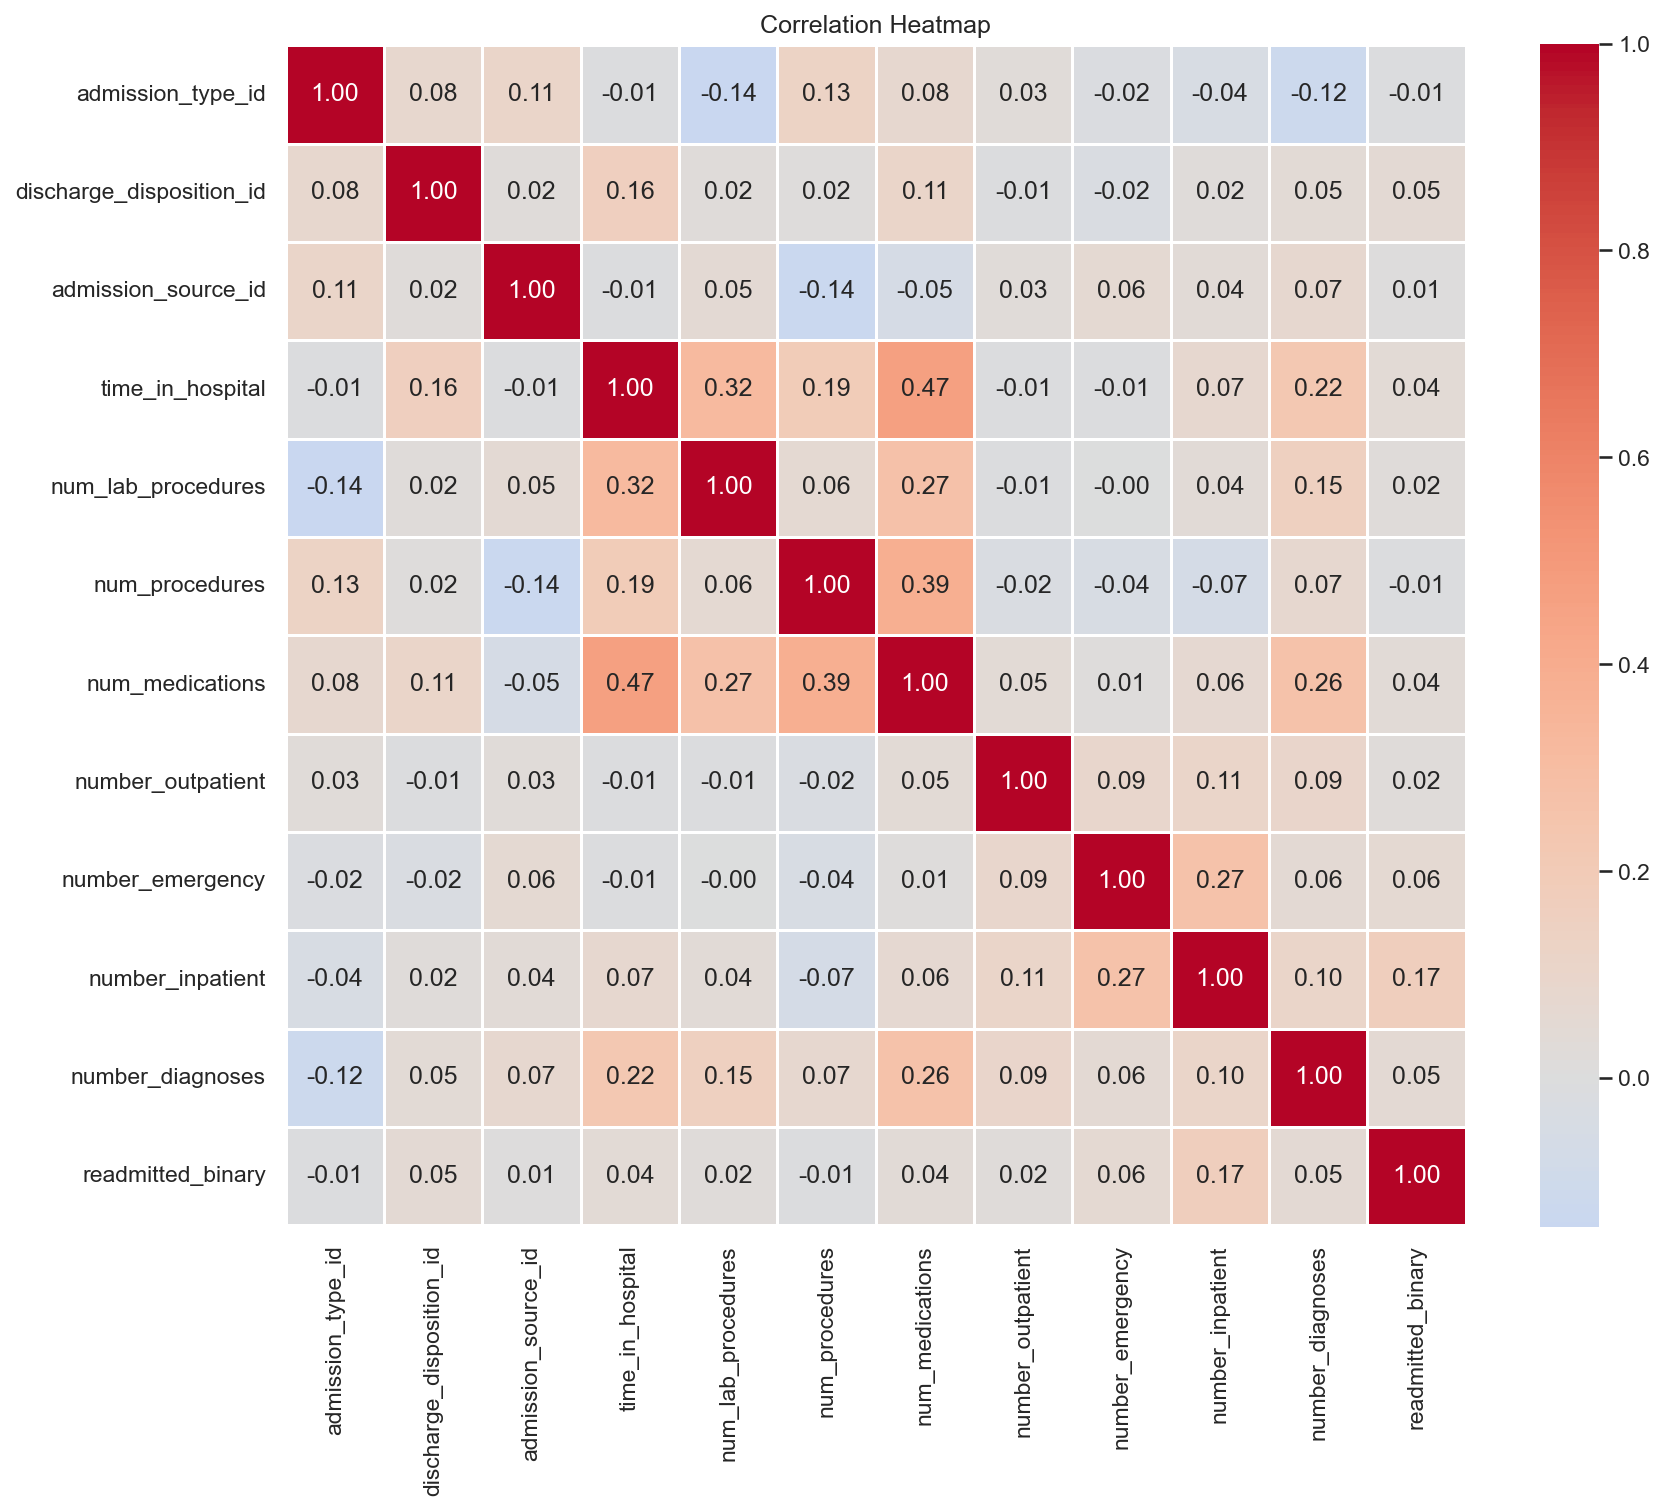
\includegraphics[width=0.5\linewidth]{figures/01_correlation_heatmap.png}
    \caption{Correlation heatmap revealing the relationships between key engineered clinical features and the readmission target variable. While this can indicate where to seek future research for causal links, we note that there is limited correlation with the target variable.}
    \label{fig:correlation_heatmap}
\end{figure}

\section{Model}
To bridge the gap between predictive accuracy and actionable Knowledge Discovery, our modeling framework benchmarks interpretable algorithms (Logistic Regression, Decision Trees) against strong opaque performers (Random Forest, Gradient Boosting). 

To fairly assess performance across algorithms, we employed a 10-Fold Stratified Cross-Validation nested scheme. The outer loop preserves genuine model evaluation, while an inner loop (5-Fold Stratified CV) facilitates hyperparameter tuning (GridSearchCV). Over-sampling the minority class is achieved locally within the CV partitions using the Synthetic Minority Over-sampling Technique (SMOTE), protecting the validation sets from data leakage. Standardized continuous attributes are likewise scaled exclusively on train folds. 

Because accuracy is heavily impacted by the dataset imbalance, evaluating the predictive quality based on a conventional accuracy metric is highly deceptive. Instead, models were assessed via AUC-ROC and AUPRC. Furthermore, we explicitly introduced a Cost-Sensitive Evaluation framework derived from business logic:
\begin{itemize}
    \item \textbf{False Negatives (Missed Readmission)}: Carry a severe penalty (e.g., -\$15,000) under the HRRP framework.
    \item \textbf{False Positives (Unnecessary Intervention)}: Carry a mild operational cost (e.g., -\$200).
    \item \textbf{True Positives}: Net a preventative benefit (-\$2,000 baseline cost for intervention instead of full readmission).
\end{itemize}
Using these assigned magnitudes, we optimize the decision thresholds. Rather than defaulting to a 0.5 probability cutoff, adjusting the threshold explicitly minimizes expected total costs.

\section{Analysis and Findings}

\begin{figure}[!ht]
    \centering
    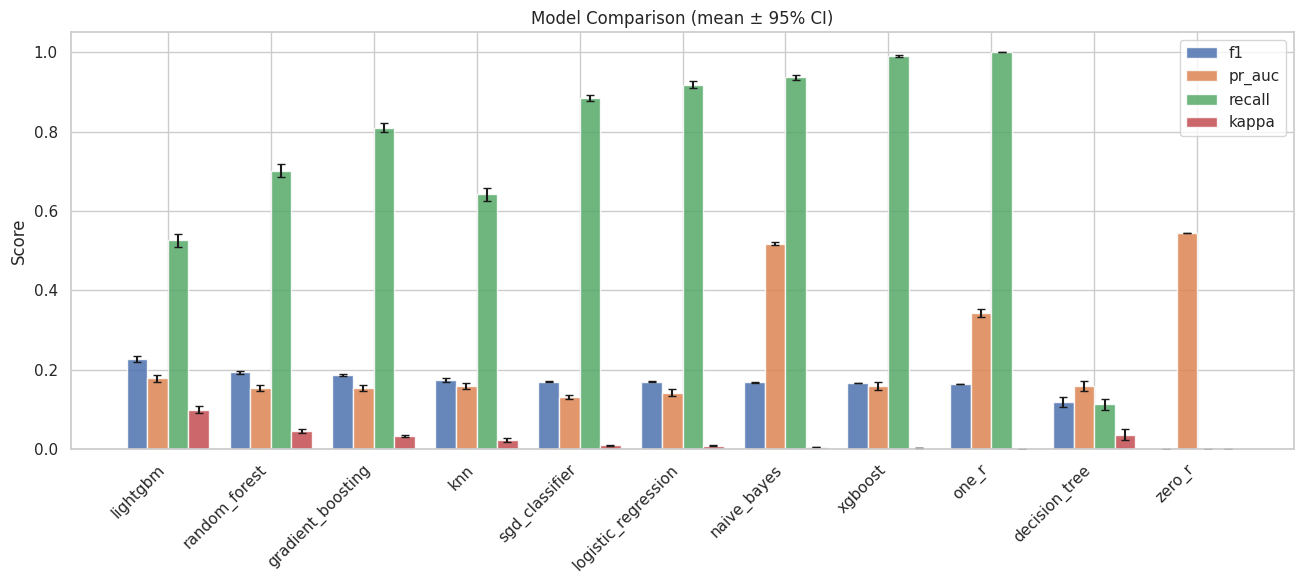
\includegraphics[width=0.7\linewidth]{figures/metrics.png}
    \caption{Performance of different models on various metrics, after applying techniques to address class imbalance. The cost-sensitive evaluation framework reveals that while some models may have similar AUC-ROC scores, their practical utility in reducing HRRP penalties can differ significantly based on their ability to capture minority class instances.}
    \label{fig:metrics}
\end{figure}

Our investigation confirmed that the intense dataset imbalance (approximately an 11:89 ratio) makes vanilla model performance misleading; zero-rule or baseline models deceptively yield 89\% accuracy without predicting a single hospitalization. The initial modeling phases underscored that the dataset is fundamentally challenging and not linearly separable. The complex, overlapping clinical profiles of the patient population meant that linear instances struggled to define clear boundaries separating the minority class. 

To combat this, we deeply invested in strategies to forcefully expose the models to the high-risk patient subset. Our pipeline explicitly tested several balancing strategies, eventually standardizing on a combination of built-in algorithm class weighting alongside fold-local over-sampling (via SMOTE). This twofold approach empowered the algorithms to learn the rare profiles safely inside the nested validation loops without causing data leakage. Furthermore, the necessary one-hot encoding of clinical categories temporarily ballooned the feature space to over 2,500 columns. To restrict model complexity and computational overhead without surrendering fidelity, we heavily utilized fold-local dimensionality reduction. We implemented L1-regularized selection and an ensemble-backed \texttt{SelectFromModel} approach, alongside PCA and \texttt{SelectKBest}. This systematically isolated the most predictive factors while aggressive algorithmic pruning shed the uninformative, sparse clinical noise.

However, moving past generic metrics provided more actionable insights. The AUC-ROC proved robust in handling class imbalance. After proper tuning and feature elimination, models began identifying valid correlative relationships in patient covariates. We found that features detailing the count of concurrent medications (\texttt{num\_medications}), changes in specific diabetic prescriptions, and historical healthcare utilization (inpatient and emergency visits) heavily govern short-term risk.

Critically, when implementing the cost-sensitive framework, tuning the decision threshold strictly below 0.5 captured far more minority class instances (increased Recall). Taking a larger volume of False Positives (spending minor sums on preventative care or phone calls) vastly outweighs missing a True Positive (a penalized HRRP readmission). 

Based on these findings, hospital administration should integrate these interpretable risk triggers directly into their Electronic Health Record (EHR) discharge workflows. Rather than presenting clinicians with an abstract probability score, the system should actively flag patients who exhibit high-risk characteristics---such as complex medication dynamics or high historical utilization---using the optimized cost-sensitive threshold. Once flagged, standard low-cost preventative protocols, such as scheduled outpatient follow-up calls or comprehensive medication reconciliations by a pharmacist, can be automatically triggered. This programmatic approach ensures that discharge resources are allocated strategically, deliberately trading inexpensive outpatient care to mitigate severe HRRP financial penalties.

\section{Conclusions}
In summary, this project shifts the focus of predicting 30-day diabetic readmissions from chasing raw accuracy to emphasizing Cost-Sensitive Knowledge Discovery. By processing the Diabetes 130-US Hospitals dataset safely and effectively treating class imbalance via SMOTE inside nested validation loops, we demonstrated how transparent, interpretable models can approach the utility of ensemble techniques. 

The explicit recommendation resulting from this process is to reject black-box probability scores in favor of transparent rule-set overlays deployed to clinicians during discharge. Optimizing decision thresholds explicitly against the profound cost disparities of Missed Readmissions (FN) versus Unnecessary Preventative Care (FP) not only mitigates HRRP penalties but directly delivers comprehensible, actionable guidelines for hospital decision-makers.

\bibliographystyle{IEEEtran}
\bibliography{references}

\end{document}